%\documentclass[11pt,a4paper]{article}
\documentclass[twocolumn]{book}
\usepackage{parskip}
\usepackage[bottom=1in]{geometry}
%%
\usepackage{multicol}
\setlength{\columnsep}{0.9cm}
\usepackage{supertabular}
\usepackage[utf8]{inputenc}
%\usepackage{geometry}   % Setup for page and paper dimensions
\usepackage{wrapfig}
\usepackage{subfigure}
\usepackage{caption}
\captionsetup{
  font=small,
  labelfont=bf,
  tableposition=top
}

\usepackage[swedish]{babel}
\usepackage{hyperref}
\hypersetup{
    colorlinks,
    citecolor=black,
    filecolor=black,
    linkcolor=black,
    urlcolor=black,
    pdfborder = {0 0 0}
}
%\usepackage{subcaption}
\usepackage{verbatimbox}
\usepackage{graphicx}   
\usepackage{lipsum}  
\usepackage{amsmath}
\usepackage{listings}   
\usepackage{tikz}
\usetikzlibrary{backgrounds,automata}
\usepackage{ifthen}
%\usepackage{pgfplots}
%\pgfplotsset{compat=newest} %<------ Here
%\usepgfmodule{plot}
\title{Övningsuppgifter Energiteknik}
\author{Lasse Karagiannis}
%\date{} % Activate to display a given date or no date (if empty),
         % otherwise the current date is printed 
\mathchardef\mhyphen="2D

%\input{insbox}
%\makeatletter
%\@InsertBoxMargin =1em
%\makeatother
\usepackage{multirow}
\begin{document}
%\maketitle
%\lipsum[1]
%\begin{multicols}{2}
\noindent\textbf{5.1-89}\hfill\break
\noindent En ideal gas genomlöper följande kretsprocess medurs:\hfil\par
\noindent\begin{tabular}{ l l  } 
1 $\rightarrow$ 2 & Uppvärmning under konstant volym\\
                  & från $t_1$ till $t_2$  \\ 
2 $\rightarrow$ 3 & Isentropisk expansion till $t_3$  \\ 
3 $\rightarrow$ 1 & Isoterm kompression till utgångs-\\
                  &punkten \\ 
\end{tabular}


Rita processen i $p$-$v$- och $T$-$s$-diagrammen. Beräkna processens termiska
verkningsgrad då $t_1=20^{\rm{o}}$C och $t_2=200^{\rm{o}}$C.

\bigskip

\begin{figure}[h]
\centering
%%%%%%%%%%%%%%%p-V-diagram
\subfigure[$p\mhyphen V$ diagram] 
{
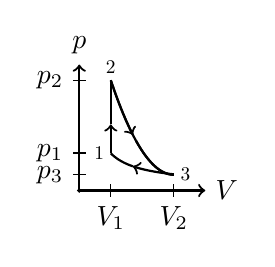
\begin{tikzpicture}[ scale=.4,baseline={(0,0)}]
%\draw (0,0) grid (4,4);
% x-axis
\draw [thick,->] (0,0) -- (4,0) node[right]{$V$};
% y-axis
\draw [thick,->] (0,0) -- (0,4) node[above] {$p$};
% x-axis label
%\node at (-0.3,4){$p$};
% y-axis label
%\node at (3.85,-0.4){$V$};
% origin point
\draw [color=black,fill=black] (0,0) circle (0.05);
%Isokor uppvärmning
\draw [thick,->](1,1.19) -- (1,2.1);
\draw [thick](1,2.1) -- (1,3.5)node[above,scale=0.7]{2};
%Isentropis expansion
\draw[ thick,domain=1:3, smooth, variable=\x, black] plot ({\x}, {(0.5+(3.5-0.5)*(abs((\x-3)/(1-3)))^2});
\draw[ thick,->,domain=1:1.7, smooth, variable=\x, black] plot ({\x}, {(0.5+(3.5-0.5)*(abs((\x-3)/(1-3)))^2});
\draw[ thick,domain=1.8:3, smooth, variable=\x, black] plot ({\x}, {(0.5+(3.5-0.5)*(abs((\x-3)/(1-3)))^2});
%Want to use the below instead
% \coordinate (A) at (1,3.5);
%\foreach \x in {1,...,3}{
%\coordinate (B) at (\x,{(0.5+(3.5-0.5)*(abs((\x-3)/(1-3)))^2});
%%\draw[thick, black] (A)--(B) ;
%\ifthenelse{\x = 2.5}{\draw[thick,->,smooth, black] (A)--(B) ;}{\draw[thick,smooth, black] (A)--(B) ;}
%\coordinate (A) at (B);
%}
%Isoterm kompression
\node[scale=0.7, right] at (3,0.5) {3};
\draw[ thick,->,domain=3:1.7, smooth, variable=\x, black] plot ({\x}, {1/\x + 0.18});
\draw[ thick,domain=1.7:1, smooth, variable=\x, black] plot ({\x}, {1/\x + 0.18}); 
\node[scale=0.7, left] at (1,1.19) {1};
%Små streck på p-axeln 
\draw  (0.2,1.19) -- (-0.2,1.19) node[left] {$p_1$};
%\node at (-1,1.19) {$p_1$};
\draw  (0.2,3.5)--(-0.2,3.5) node[left] {$p_2$};
\draw  (0.2,0.5)--(-0.2,0.5) node[left] {$p_3$};
%\node at (-1,3.5)  {$p_2$};
%Små streck på V-axeln
\draw (1,0.2) -- (1,-0.2) node[below]{$V_1$};
%\node at (1, -1) {$V_1$};
\draw (3,0.2) -- (3,-0.2) node[below]{$V_2$};;
%\node at (2.5,-1) {$V_2$};
\end{tikzpicture}
}
%      \caption{Mät2 }
\label{fig1}
%  
%%%%%%%%%%%%%%%%%%%%%%%%%%%T-s-diagram
\subfigure[$T\mhyphen s$ diagram]
{
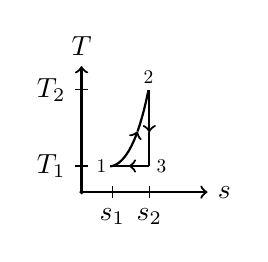
\begin{tikzpicture}[scale=.4,baseline={(0,0)}]
%\begin{tikzpicture}[show background rectangle, scale=.5]

%\draw (0,0) grid (4,4);
% x-axis
\draw [thick,->] (0,0) -- (4,0) node[right]{$s$};
% y-axis
\draw [thick,->] (0,0) -- (0,4) node[above]{$T$};
% x-axis label
%\node at (-0.3,4){$T$};
% y-axis label
%\node at (4,-0.3){$s$};
%origin point
\draw [color=black,fill=black] (0,0) circle (0.05);
%Isokor uppvärmning
\node[scale=0.7,left] at (1,0.83){1};
\draw[ ->,rotate=7,thick,domain=1:2, smooth, variable=\x, black] plot ({\x}, {(0.7 + (\x-1)^2});
\draw[ rotate=7,thick,domain=2:2.5, smooth, variable=\x, black] plot ({\x}, {(0.7 + (\x-1)^2}) node[scale=0.7,above]{2};
%Isentropis expansion
\draw [thick,->] (2.15,3.25) -- (2.15,1.9);
\draw [thick] (2.15,1.9) -- (2.15,0.83) node[scale=0.7,right]{3};
%Isoterm kompression
\draw [thick,->] (2.15,0.83) -- (1.5,0.83);
\draw [thick] (1.5,0.83) -- (0.98,0.83);
%Små streck på T-axeln 
\draw  (0.2,0.83) -- (-0.2,0.83) node[left] {$T_1$};
%\node at (-1,0.83) {$T_1$};
\draw (0.2,3.25) -- (-0.2,3.25) node[left] {$T_2$} ;
%\node at (-1,3.25)  {$T_2$};
%Små streck på s-axeln
\draw (0.98,0.2) -- (0.98,-0.2) node[below] {$s_1$};
%\node at (0,98, -1) {$s_1$};
\draw (2.15,0.2) -- (2.15,-0.2) node[below] {$s_2$};
%\node at (2.5,-1) {$s_2$};


%Pilar
%\usetikzlibrary {arrows.meta}
%\draw [arrows ={-Stealth[scale=1]}] (1.5,2.5) -- (1.5,1.9);
%\draw [arrows ={-Stealth[scale=1]}] (1.75,1.5) -- (1.75,1.0);
%\path (1.2,2.8) node  {$q_{till}$};
%\path (1.6,0.4) node  {$q_{\textit{bort}}$}; 

\end{tikzpicture}
}
%    \caption{Mät 2}
\label{fig2}
%\caption{Anpassning av $n$ i $p=\frac{C}{V^n}$}
\end{figure}

Den teoretiska termiska verkningsgraden definieras enligt
%\begin{wrapfigure}[5]{l}{0cm}
\begin{flalign*}
\eta_t &=\frac{q_{tillf}-|q_{bortf}|}{q_{tillf}} &\\
       &=1-\frac{|q_{bortf}|}{q_{tillf}}
\end{flalign*}
%\end{wrapfigure}
Avseende $q_{tillf}$ som ju är $q_{12}$ så rör vi oss till höger i $T\mhyphen s$ diagrammet.
Integralen blir då positiv.\\
\begin{flalign*}
q_{12}&=\int_1^2 T\cdot ds &
\end{flalign*}
Värmemängdsändringen är således ändringen av den inre energin.
\begin{flalign*}
q_{12}&=\bar{c}_v\cdot(T_2)-T_1) &
\end{flalign*}
Problemställningen talar om en ideal gas men ger inget värde.
För en enatomig ideal gas gäller 
\begin{flalign*}
c_v&=\frac{3}{2}R &\\
c_p&=\frac{5}{2}R
\end{flalign*}
För en tvåatomig ideal gas gäller 
\begin{flalign*}
c_v&=\frac{5}{2}R &\\
c_p&=\frac{7}{2}R
\end{flalign*}
Vi antar att det rör sig om en enatomig ideal gas. Således skriver vi
\begin{flalign*}
q_{tillf}&=\frac{3}{2}R\cdot(T_2-T_1) &\\
         &=\frac{3}{2}R\cdot(200-20)&
\end{flalign*}
Värme bortförs under isotermen eftersom integrationsriktningen är omvänd, 
$q_{13}<0$, vilket också stämmer rent intuitivt. Om vi komprimerar gasen så stiger temperaturen men för att hålla
temperaturen konstant så måste vi hela tiden bortföra värmeenergi under komprimeringsprocessen.
Eftersom temperaturen på gasen inte ändras så ändras inte
inre energin $u_3-u_1=0$.
Ändringen av värmeenergin $q_{31}$ blir alltså lika med volymändringsarbetet $w_{31}$
$q_{31}=w_{31}$. Volymändringsarbetet är per definition
\begin{flalign*}
w_{31}&=\int_3^1 p\cdot dv &\\
      &=\int_3^1\frac{R\cdot T}{v}dv &\\
      &=R\cdot T\cdot ln(\frac{v_1}{v_3}) &\\
q_{bort}&=R\cdot T\cdot ln(\frac{v_1}{v_3}) &
\end{flalign*}
Vi har dock ingen information om värden $p$ och $v$ sådant att vi kan räkna ut detta förutom att
vi vet att för en isoterm så gäller $p_1\cdot V_1 = p_3\cdot V_3$
Vi ser dock att arean under kurvan i $T\mhyphen s$ diagrammet är en rektangel som vi
enkelt kan beräkna arean av såsom $(s_1 - s_3)\cdot T_1$.\\ Entropiändringen är
\begin{flalign*}
\int_3^1 ds &=\int_3^1 \frac{dQ}{T}&\\
s_1 -s_3 &= \int_3^1 \frac{1}{T} du + p\cdot dv &\\
         &= \int_3^1 \frac{1}{T} 0 + p\cdot dv &\\
         &=\int_3^1\frac{1}{T}\frac{R\cdot T}{v}dv &\\
         &=R\cdot ln(\frac{v_1}{v_3}) &\\
         &=R\cdot ln(\frac{v_1}{v_3}) &
\end{flalign*}
Denna informationen ger ingenting men vi vet att
$s_2=s_3$ så vi kan faktiskt räkna ut den sökta differensen
från isokor-processen
\begin{flalign*}
\int_1^2 ds &=\int_1^2 \frac{dQ}{T}&\\
s_2 -s_1 &= \int_1^2 \frac{1}{T} du + p\cdot dv &\\
         &= \int_1^2 \frac{1}{T} du + p\cdot 0 &\\
         &=\int_3^1\frac{1}{T}c_v\cdot dT &\\
         &=c_v\cdot ln(\frac{T_2}{T_1}) &\\
         &=\frac{3}{2}R\cdot ln(\frac{(273+200)}{273+20}) &\\
         &=\frac{3}{2}R\cdot 0.478922779
\end{flalign*}
$s_1 - s_3 =-(s_2 -s_1)=-\frac{3}{2}R\cdot 0.478922779$\\
Detta ger att
\begin{flalign*}
|q_{bort}|&=T_1\cdot \frac{3}{2}R\cdot 0.478922779\\&
\end{flalign*}
Vilket ger oss
\begin{flalign*}
\eta_t &=1-\frac{|q_{bortf}|}{q_{tillf}} &\\
       &=1-\frac{T_1\cdot \frac{3}{2}R\cdot 0.478922779}{\frac{3}{2}R\cdot(200-20)} &\\
       &=1 -\frac{(273+20)\cdot 0.478922779}{(200-20)} &\\
       &=1-0.779579858 = 0.220420142
\end{flalign*}
Korrekt svar måste anges med korrekt antal värdesiffror. Talet 200 har tre värdesiffror
och 20 har två värdesiffror. Talet 20 blir då bestämmande och svaret måste anges med
två värdesiffror. Således $\eta_t = 0.22$

%%%%%%%%%%%%%%%%%%%%%%%%%%%%%%%%%%%%%%%%%%%%%%%%%%%%%%%%%%%%%%%%%%%%%%%%%%%%%%%%%%%%
%%%%%%%%%%%%%%%%%%%%%%%%%%%%%%%%%%%%%%%%%%%%%%%%%%%%%%%%%%%%%%%%%%%%%%%%%%%%%%%%%%%%
%%%%%%%%%%%%%%%%%%%%%%%%%%%%%%%%%%%%%%%%%%%%%%%%%%%%%%%%%%%%%%%%%%%%%%%%%%%%%%%%%%%%
%%%%%%%%%%%%%%%%%%%%%%%%%%%%%%%%%%%%%%%%%%%%%%%%%%%%%%%%%%%%%%%%%%%%%%%%%%%%%%%%%%%%
%%%%%%%%%%%%%%%%%%%%%%%%%%%%%%%%%%%%%%%%%%%%%%%%%%%%%%%%%%%%%%%%%%%%%%%%%%%%%%%%%%%%
%%%%%%%%%%%%%%%%%%%%%%%%%%%%%%%%%%%%%%%%%%%%%%%%%%%%%%%%%%%%%%%%%%%%%%%%%%%%%%%%%%%%
\bigskip
\noindent\textbf{5.1-94}\hfill\break
\noindent En ideal gas genomlöper följande kretspro-\\
cess medudurs
\begin{table}[ht]
\noindent\begin{tabular}{ l l  } 
1 $\rightarrow$ 2 & Isentropisk kompression\\
2 $\rightarrow$ 3 & Tryckökning vid konstant volym  \\ 
3 $\rightarrow$ 4 & Polytropisk expansion $(n=1.2)$.\\
4 $\rightarrow$ 1 & Tryckminskning vid konstant volym.\\                
\end{tabular}
\end{table}

Rita processen i $p$\,-$V$- och $T$-$s$-diagrammen.
Bestäm termiska verkningsgraden då $T_1=300$K. $T_3=700$K, $T_4=500K$ och $\kappa=1.4$.
\bigskip

\begin{figure}[h]
\centering
%%%%%%%%%%%%%%%p-V-diagram
\subfigure[$p\, \mhyphen V$ diagram] 
{
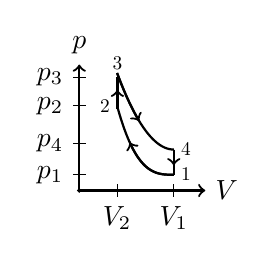
\begin{tikzpicture}[ scale=.4,baseline={(0,0)}]
%\draw (0,0) grid (4,4);
% x-axis
\draw [thick,->] (0,0) -- (4,0) node[right]{$V$};
% y-axis
\draw [thick,->] (0,0) -- (0,4) node[above] {$p$};
% origin point
\draw [color=black,fill=black] (0,0) circle (0.05);

%Isentropisk kompression från x1=3.5, y1=0.5 till x2=0.6, y2=2
%y= y0+(y1-y2)*abs((x-x2)/(x2-x1))^n
%\draw[ thick,->,domain=3.5:0.6, smooth, variable=\x, black] plot ({\x}, {0.716*abs(\x-3.5)^1.4 -0.5});
%\draw[ thick,domain=3.5:0.6, smooth, variable=\x, black] plot ({\x}, {(0.5+(2-0.5)*(abs((\x-0.6)/(0.6-3.5)))^2}) node[scale=0.7, left]{2};
\draw[ thick,domain=3:1.2, smooth, variable=\x, black] plot ({\x}, {(0.5+(3.5-0.5)*(abs((\x-3)/(1-3)))^3}) node[scale=0.7, left]{2};
\draw[ thick,->,domain=3:1.6, smooth, variable=\x, black] plot ({\x}, {(0.5+(3.5-0.5)*(abs((\x-3)/(1-3)))^3});
%Ticks on p-axis
\draw (0.2,{(0.5+(3.5-0.5)*(abs((3-3)/(1-3)))^3}) -- (-0.2,{(0.5+(3.5-0.5)*(abs((3-3)/(1-3)))^3}) node[left]{$p_1$};
\draw (0.2,{(0.5+(3.5-0.5)*(abs((1.2-3)/(1-3)))^3}) -- (-0.2,{(0.5+(3.5-0.5)*(abs((1.2-3)/(1-3)))^3}) node[left]{$p_2$};
%Ticks on V-axis
\draw(3,0.2)--(3,-0.2) node [below] {$V_1$};
\draw(1.2,0.2)--(1.2,-0.2) node [below] {$V_2$};


%Isokor uppvärmning (Tryckökning)
%x1=1.2, y1=1.958 till x2=1.2, y2=3.6
\draw[thick] (1.21,2.6)--(1.21,3.6) node[scale=0.7, above]{3};
\draw[thick,->] (1.21,2.6)--(1.21,3.2);

\draw (0.2,3.6)--(-0.2,3.6) node[left]{$p_3$};

%Polytropisk expansion
%x1=0.6, y1=3.6 till x2=3.5 y2 = 1.5
\draw[ thick,domain=1.2:3, smooth, variable=\x, black] plot ({\x}, {(1.30+(3.5-0.5)*(abs((\x-3)/(1-3)))^2}) node[scale=0.7, right]{4};
\draw[ thick,->,domain=1.2:1.9, smooth, variable=\x, black] plot ({\x}, {(1.30+(3.5-0.5)*(abs((\x-3)/(1-3)))^2});

\draw (0.2,{(1.30+(3.5-0.5)*(abs((3.5-3)/(1-3)))^2} ) -- (-0.2,{(1.30+(3.5-0.5)*(abs((3.5-3)/(1-3)))^2} ) node[left] {$p_4$};

%Isokor nedkylning (tryckminskning)
%x1=3.0 y1 = 1.5 till x1=3.0, y2=0.5
\draw[thick] (3.0,1.3)--(3.0,0.5) node[scale=0.7, right]{1};
\draw[thick,->] (3.0,1.3)--(3.0,0.8);

%Små streck på p-axeln 
%\draw  (0.2,1.19) -- (-0.2,1.19) node[left] {$p_1$};
%\node at (-1,1.19) {$p_1$};
%\draw  (0.2,3.5)--(-0.2,3.5) node[left] {$p_2$};
%\draw  (0.2,0.5)--(-0.2,0.5) node[left] {$p_3$};
%\node at (-1,3.5)  {$p_2$};
%Små streck på V-axeln
%\draw (1,0.2) -- (1,-0.2) node[below]{$V_1$};
%\node at (1, -1) {$V_1$};
%\draw (3,0.2) -- (3,-0.2) node[below]{$V_2$};;
%\node at (2.5,-1) {$V_2$};
\end{tikzpicture}
}
%      \caption{Mät2 }
\label{fig3}
%  
%%%%%%%%%%%%%%%%%%%%%%%%%%%T-s-diagram
\subfigure[$T\mhyphen s$ diagram]
{
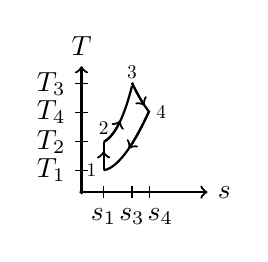
\begin{tikzpicture}[scale=.4,baseline={(0,0)}]
%\begin{tikzpicture}[show background rectangle, scale=.5]

%\draw (0,0) grid (4,4);
% x-axis
\draw [thick,->] (0,0) -- (4,0) node[right]{$s$};
% y-axis
\draw [thick,->] (0,0) -- (0,4) node[above]{$T$};
% x-axis label
%\node at (-0.3,4){$T$};
% y-axis label
%\node at (4,-0.3){$s$};
%origin point
\draw [color=black,fill=black] (0,0) circle (0.05);
%Isentropisk kompression
%x1=1.2, y1=1.958 till x2=1.2, y2=3.6
\draw[thick] (0.7,0.7)--(0.7,1.6) node[scale=0.7, above]{2};
\draw[thick,->] (0.7,0.7)--(0.7,1.3);

\draw (0.2,0.7)--(-0.2,0.7) node[left]{$T_1$};
\draw (0.7,0.2)--(0.7,-0.2) node[below]{$s_1$};

\draw (0.2,1.6)--(-0.2,1.6) node[left]{$T_2$};


%Isokor uppvärmning
%Isokor uppvärmning
%\node[scale=0.7,left] at (1,0.83){1};
\draw[ ->,rotate=7,thick,domain=0.9:1.5, smooth, variable=\x, black] plot ({\x}, {(1.46 + (\x-0.7)^2});
\draw[ rotate=7,thick,domain=0.9:2, smooth, variable=\x, black] plot ({\x}, {(1.46 + (\x-0.7)^2}) node[scale=0.7,above]{3};

\draw (0.2,{(2.8 + (1.5-0.7)^2})--(-0.2,{(2.8 + (1.5-0.7)^2}) node[left]{$T_3$};
\draw (1.6,0.2)--(1.6,-0.2) node[below]{$s_3$};

%Polytrop expansion n<kappa
%\node[scale=0.7, right] at (2,3.5);
%y= y0+(y1-y2)*abs((\x-x2)/(x2-x1))^n (2,3.15) -> (3.5,1.5)
%\draw[ thick,domain=1.2:1.9, smooth, variable=\x, black] plot ({\x}, {y0+(y1-y2)*abs((\x-x2)/(x2-x1))^n});
%\draw[ thick,domain=1.7:2.5, smooth, variable=\x, black] plot ({\x}, {1.5+(3.15-1.5)*abs((\x-3.5)/(3.5-2))^2});
\draw[ thick,domain=1.6:2.15, smooth, variable=\x, black] plot ({\x}, {(2+(3.5-0.5)*(abs((\x-3)/(1-3)))^2}) node[scale=0.7, right]{4};
\draw[ thick,->,domain=1.6:2, smooth, variable=\x, black] plot ({\x}, {(2+(3.5-0.5)*(abs((\x-3)/(1-3)))^2});
%\draw[ thick,->,domain=3:1.6, smooth, variable=\x, black] plot ({\x}, {(0.5+(3.5-0.5)*(abs((\x-3)/(1-3)))^2})

\draw (0.2,{(2+(3.5-0.5)*(abs((2.15-3)/(1-3)))^2})--(-0.2,{(2+(3.5-0.5)*(abs((2.15-3)/(1-3)))^2}) node[left]{$T_4$};
\draw (2.15,0.2)--(2.15,-0.2);
\node (A) at (2.5,-0.2)[below]{$s_4$};

%Isokor nedkylning
%\node[scale=0.7,left] at (1,0.83){1};
\draw[ ->,rotate=0,thick,domain=2.15:1.5, smooth, variable=\x, black] plot ({\x}, {(0.7 + (\x-0.7)^1.7});
\draw[ rotate=0,thick,domain=2.15:0.7, smooth, variable=\x, black] plot ({\x}, {(0.7 + (\x-0.7)^1.7}) node[scale=0.7, left]{1};



%Pilar
%\usetikzlibrary {arrows.meta}
%\draw [arrows ={-Stealth[scale=1]}] (1.5,2.5) -- (1.5,1.9);
%\draw [arrows ={-Stealth[scale=1]}] (1.75,1.5) -- (1.75,1.0);
%\path (1.2,2.8) node  {$q_{till}$};
%\path (1.6,0.4) node  {$q_{\textit{bort}}$}; 

\end{tikzpicture}
}
%    \caption{Mät 2}
\label{fig4}
%\caption{Anpassning av $n$ i $p=\frac{C}{V^n}$}
\end{figure}

Den teoretiska termiska verkningsgraden definieras enligt
%\begin{wrapfigure}[5]{l}{0cm}
\begin{flalign*}
\eta_t &=\frac{q_{tillf}-|q_{bortf}|}{q_{tillf}} &\\
       &=1-\frac{|q_{bortf}|}{q_{tillf}}
\end{flalign*}




%\end{multicols}
%\listoffigures
%\listoftables
%\tableofcontents

\end{document}
